\chapter{Formal background}
\label{chapters:formal-background}

This chapter proposes modifications to the framework layers introduced by previous tools \textit{XCase} and \textit{eXolutio} and formally describes them. Some problems are further analyzed as the reasoning depends on the framework structure and not just user requirements.

As mentioned in the previous chapter, not everything has been implemented yet due to the complexity of the problem. Nevertheless, it is crucial to properly design and plan everything in advance to minimize the technical debt.

\bigskip

In contrast with the approach introduced in \textit{XCase} and \textit{eXolutio} tools, the process of creating the domain ontology is moved from the application to the external tools. The application then only uses those ontologies if required.

To fulfill the introduced requirements, we have modified the previously introduced five-level framework in the following way:
\begin{itemize}
    \item We have added a new top-most level called \textbf{CIM} (from \textit{Computational Independent Model}). CIM represents the remote ontology on the web according to \autoref{requirement:ontologies-on-the-web}. Although the level is part of the framework design, it is important to stress that it has no direct representation in the tool as it represents data on the web. Because we suppose ontologies respect LD principles, we can see them as a single graph, not multiple independent sources.
    \item Previous \textbf{PIM} layer is used as a copy of the CIM layer, and only the necessary entities are copied to it. This approach is compatible with the design of the previous tools, which used PIM as the source of the ontology.
\end{itemize}

This modification brings several advantages:
\begin{enumerate}
    \item As the ontology is copied, this allows us to use the tool seamlessly without depending on the ontology. We can generate artifacts and modify the schema. Only the operations related to directly using the ontology depend on CIM.
    \item The mechanism that derives a list of changes during the evolution (see \autoref{requirement:evolution}) may use the PIM layer as a comparison.
    \item The layer still separates the ontology from the rest of the model, simplifying the design of the whole framework. For example, the other layers may refer to information in PIM.
\end{enumerate}

PSM, as a second level from the five-level framework, then represents the general schema.

In the previous chapter, we defined data specification as a project containing multiple schemas, configurations for generators, and metadata, such as a list of reused specifications. This would mean that individual PSMs belong to a concrete data specification. To simplify things, we say that exactly one PIM is part of the specification as well.

\begin{figure}[h]\centering
    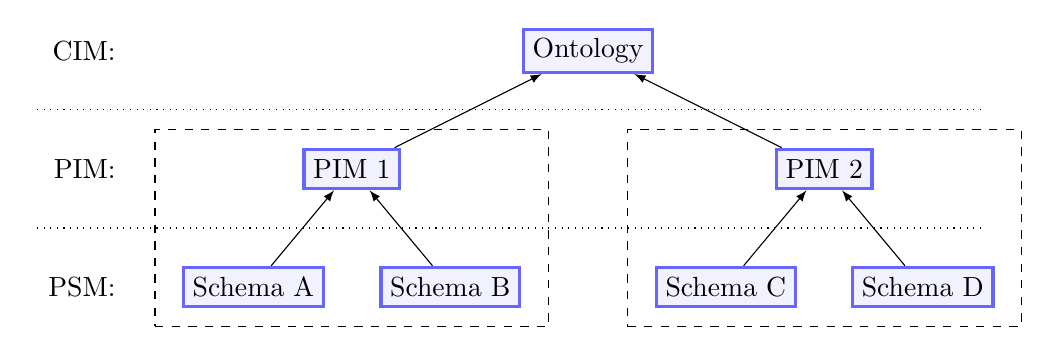
\begin{tikzpicture}[
        squarednode/.style={rectangle, draw=blue!60, fill=blue!5, very thick, minimum size=5mm},
    ]
        %Nodes
        \node[squarednode] (cim) at (0,0) {Ontology};
        \node[squarednode] (pim1) at (-3,-1.5) {PIM 1};
        \node[squarednode] (pimn) at (3,-1.5) {PIM 2};

        \node[squarednode] (psma) at (-4.25,-3) {Schema A};
        \node[squarednode] (psmb) at (-1.75,-3) {Schema B};

        \node[squarednode] (psmc) at (1.75,-3) {Schema C};
        \node[squarednode] (psmd) at (4.25,-3) {Schema D};

        \node (psm_t)[text width=1cm,align=right] at (-6.5,0) {{CIM:}};
        \node (pim_t)[text width=1cm,align=right] at (-6.5,-1.5) {{PIM:}};
        \node (schema_t)[text width=1cm,align=right] at (-6.5,-3) {{PSM:}};

        %Lines
        \draw[-latex] (psma) -- (pim1);
        \draw[-latex] (psmb) -- (pim1);
        \draw[-latex] (psmc) -- (pimn);
        \draw[-latex] (psmd) -- (pimn);
        \draw[-latex] (pim1) -- (cim);
        \draw[-latex] (pimn) -- (cim);

        %\path(psmc) edge [-latex,out=135, in=315]  (psmb);

        \node[dashed, draw=black, minimum width=5cm, minimum height=2.5cm] at (-3,-2.25) {};
        \node[dashed, draw=black, minimum width=5cm, minimum height=2.5cm] at (3,-2.25) {};


        % separators
        \foreach \x in {0,...,1}{
            \draw [dotted] (-7,-0.75-1.5*\x) -- (5,-0.75-1.5*\x);
        }
    \end{tikzpicture}
    \caption{Schema of the new framework structure (without the lower levels containing artifacts). The topmost level represents the ontology, then different PIMs serve as copies of the ontology for different data specifications that are represented by dashed rectangles. The third level represents the general schemas.} % Schema C shows a proposition for schema extending and is described later in the thesis.
\end{figure}

\section{Conceptual levels}

We will start by defining PIM, as the definition of CIM depends on it.

\begin{definition}[PIM] PIM is a quadruple $C=(C_\textrm{c}, C_\textrm{attr}, C_\textrm{assoc}, C_\textrm{end})$ of sets of classes, attributes, associations and association ends, respectively (we will call them as entities), with a set of annotation functions such that:
    \begin{itemize}
        \item Attribute $a \in C_\textrm{attr}$ belongs to exactly one class $c \in C_\textrm{c}$, which is denoted by annotation function $\textrm{class}: C_\textrm{attr} \rightarrow C_\textrm{c}$ as $\textrm{class}(a)=s$.
        \item Association $r \in C_\textrm{assoc}$ has a tuple of two distinct associations ends denoted by $\textrm{end}: C_\textrm{assoc} \rightarrow C_\textrm{end}\times C_\textrm{end}$. Each association end belongs to exactly one association. Each association end has one class denoted by $\textrm{class}: C_\textrm{assoc} \rightarrow C_\textrm{c}$.
    \end{itemize}

    PIM entities can be decorated by other various semantic and syntactic annotations. We do not require that an annotation must be defined for every entity if not stated otherwise.

    \begin{itemize}
        \item Classes, attributes, associations, and association ends may have title and description, or potentially other describing properties that are not directly used in schema generation. However, the title may be used to propose the naming of entities' labels at the PSM level. (For example $\textrm{title}(c)="\textrm{Tourist destination}"@en$)
        \item Each class have a set of classes that they extends by annotation $\textrm{extends}: C_\textrm{c} \rightarrow \mathcal{P}(C_\textrm{c})$. (see \autoref{requirement:inheritance})
        \item Attributes and association ends have cardinalities $\textrm{card}_{\textrm{min}}: C_\textrm{attr} \cup C_\textrm{end} \rightarrow \mathds{N}_0$ and $\textrm{card}_{\textrm{max}}: C_\textrm{attr} \cup C_\textrm{end} \rightarrow \mathds{N} \cup \{\infty\}$, where $\textrm{card}_{\textrm{min}}(i) \leq \textrm{card}_{\textrm{max}}$, where the comparison operator works same as in the extended real number system.
        \item Attributes have data types $\textrm{datatype}: C_\textrm{attr} \rightarrow D$ where $D$ is a set of data types, usually specified by a IRI.
    \end{itemize}
\end{definition}

The purpose of annotations is to bring additional information to the model that is not essential for the generation. As we stated in the previous chapter, there are various ontologies, and some of them may lack the support of some construct. We have already mentioned that RDFS does not allow naming the reverse direction of an association. Some ontologies may not support cardinalities or inheritance (although most of them do). Similarly, some artifacts may not use all the information from PIM. For example, data transformations do not need a title and description to work with.

We do not provide a complete list of all annotations as the intention is to let programmers use their own if necessary, either when creating a new generator or adding support for the new format of an ontology.

The purpose of PIM entities should be clear as we have described all important concepts in \autoref{chapters:analysis}.

\begin{figure}[h!]\centering
\centering
\begin{tikzpicture}[]
    \node[typeclass] (goods) {\textbf{class}\\$title$: Goods\\$description$: Represents goods\\that can be bought.};
    \node[typeattribute] (title) at (6,0) {\textbf{attribute}\\$title$: title\\$type$: xs:string\\$cardinality$: 1..1};

    \node[typeclass] (variantc) at (0,-7.5) {\textbf{class}\\$title$: Goods variant\\$description$: Variant of good, such\\as color or material.};

    \node[typeclass] (food) at (-3,-4-0.125+1) {\textbf{class}\\$title$: Food\\$description$: Goods\\that are edible.};

    \draw[-latex] (title) -- node[below]{$class$} (goods);
    \draw[-latex] (food) -- node[right]{$extends$} (goods);

    \begin{scope}[transform canvas={xshift=1.5cm}]
        \node[typeassociation] (variant) at (5,-4-0.125) {\textbf{association}};
        \node[typeassociationend] (varianta) at (0,-3.25) {\textbf{association end}\\$title$: is variant of\\$card_{min}$: 1\\$card_{max}$: 1};
        \node[typeassociationend] (variantb) at (0,-5) {\textbf{association end}\\$title$: has variant};

        \draw[-latex] (varianta) -- node[right]{$class$} (goods);
        \draw[-latex] (variantb) -- node[right]{$class$} (variantc);
        \draw[-latex] (variant) -- node[above]{$end[0]$} (varianta);
        \draw[-latex] (variant) -- node[below]{$end[1]$} (variantb);
    \end{scope}

    \end{tikzpicture}

  \caption{Example of the PIM model shown as a graph. Rectangles represent entities. An Italic font either inside the rectangle or on the arrow represents the given annotation function with the given value.}
  \label{figure:pim-example}
\end{figure}

Because during the modeling process, CIM (specifically ontologies under different formats) is being copied to PIM, it would make sense to define the CIM in a way that is compatible with PIM.

First, we need to define an interpretation that will be used to connect entities from PIM with those in CIM.

\begin{definition}[interpretation]
    Let us have an annotation $\textrm{interpretation}: E \rightarrow \mathcal{I} \cup \{\emptyset\}$ from all entities to $\mathcal{I}$, set of CIM entities. We say that PIM entity $I$ is interpreted if and only if annotation $\textrm{interpretation}(I) \neq \emptyset$.
\end{definition}

\begin{definition}[CIM]
    CIM $O$ is an ontology for which function \textbf{CIM adapter} $A$ exists, such that $A(O) = C$ is a valid PIM, where every PIM class, attribute, and association has a different defined interpretation representing the CIM entity and that interpretation is stable over time. That means if the CIM entity is changed but still represents the semantically same thing, then the interpretation of the corresponding PIM entity shall stay the same.
\end{definition}

The definition tells us that the CIM can be viewed as a PIM where with interpretation as a pointer to the original thing in the ontology. In practice, it is the IRI of the entity in the ontology.

If the CIM changes, entities shall keep their original IRIs to stress that the given entity is semantically still the same. Only the representation may have changed. This will help us, for example, to detect changes and properly propagate them in the model.

For simplification, in the rest of the thesis, we may omit that CIM \textit{needs to be translated} to PIM and suppose that it is already in PIM-like format.

The definition does not require association ends to be interpreted as some ontologies consider the whole association as a single entity. Nevertheless, each association end belongs to its association which is interpreted. Hence the link to CIM exists.

\section{Structural level}

Ontology is represented on conceptual levels on CIM and PIMs. The constructed schemas then belong to the structural level. During the analysis of \autoref{requirement:general-schema} we have already decided on the hierarchical structure of the general schema as our target schemas also have a hierarchical structure.

We will introduce PSM (platform-specific) level to represent the schemas. PSM level is highly inspired by the PSM level from the previous tools, but we must take into account different serialization formats PSM level is generated into.

\begin{definition}[PSM]
    PSM is a tuple $S=(S_{\textrm{r}}, S_{\textrm{c}}, S_{\textrm{ref}}, S_{\textrm{or}}, S_{\textrm{attr}}, S_{\textrm{end}}, S_{\textrm{incl}})$ with a set of annotation functions such that:
    \\(let $C:=S_{\textrm{c}}\cup S_{\textrm{ref}}\cup S_{\textrm{or}}$ be a set of objects and $P:=S_{\textrm{attr}}\cup S_{\textrm{end}}\cup S_{\textrm{incl}}$ set of properties)
    \begin{itemize}
        \item $S_{\textrm{r}} \neq \emptyset$, $S_{\textrm{r}} \in C^n$ is a tuple objects that are schema roots

        \item $S_{\textrm{c}}$ is a set of classes with annotation function $\textrm{parts}: S_{\textrm{c}} \rightarrow P^n$ that returns a tuple of class properties

        \item $S_{\textrm{ref}}$ is set of all references to other PSMs with annotation function $\textrm{ref}: S_{\textrm{ref}} \rightarrow \mathcal{S} \times \mathcal{S}_{\textrm{r}}$ that returns the referenced PSM and one of its root objects

        \item $S_{\textrm{or}}$ is a set of ORs with annotation function $\textrm{choices}: S_{\textrm{or}} \rightarrow \mathcal{P}(C)$ that returns the set of all possible choices of the OR

        \item $S_{\textrm{attr}}$ is set of attributes with annotation function $\textrm{technicalLabel}: S_{\textrm{attr}} \rightarrow \textrm{string}$ that returns the label of the attribute

        \item $S_{\textrm{end}}$ is a set of association ends with two annotation functions (i)\\$\textrm{technicalLabel}: S_{\textrm{end}} \rightarrow \textrm{string}$ that returns the label of the association and (ii) $\textrm{end}: S_{\textrm{assoc}} \rightarrow C$ that returns the associated object

        \item $S_{\textrm{incl}}$ is a set of all includes with annotation function $\textrm{includes}: S_{\textrm{incl}} \rightarrow C$ that returns the included class
    \end{itemize}
\end{definition}

The definition puts together the findings from the previous chapter, where we analyzed the structure and individual concepts of the general schema. The definition re-introduces well-known terms from PIM, such as class, attribute, and association end. Association itself has no counterpart in PSM as we are only interested in one specific direction. References are a necessary concept for the implementation part as their meaning is to reference outside of the PSM, whether referring to entities inside PSM is implicit. As decided, class-level OR is used to support disjunction, hence belonging to object types that can be associated and placed as schema roots.

We allow multiple roots for a single schema for advanced cases, such as creating a database model of multiple tables. For most schemas, however, only one root is allowed. Hence, the general schema with root $R$ means PSM $S$ with a single root $S_{\textrm{c}} = (R)$ with all other entities that are part of the chain originating from the class.

Although it may seem that the PSM is a forest (tree for every root), the PSM is neither DAG nor a connected graph. We have already discussed the include construct (see \autoref{fig:cartesian-product:include}) as it takes properties from another existing class, hence creating a diamond shape in the graph. We also did not restrict that two different association ends may point to the same object. Nevertheless, we also allow oriented cycles. For example, a class may have an association end referencing the class itself. This allows us to design schemas for data structures containing, for example, serialized trees, as a tree can be arbitrarily deep.

\medskip

To keep the relation between entities from PSM and PIM, we will introduce the same concept of interpretation for PSM with a slightly different meaning. On PIM, interpretation means that the entities are de facto the same. On PSM, however, we need to say that the given PSM entity is only semantically the same as the corresponding PIM entity. Nevertheless, besides the semantic meaning, the interpretation is the concept.

\begin{definition}[interpretation on PSM]
    Let us have an annotation $\textrm{interpretation}$ defined as follows on the set of PSM classes $S_{\textrm{c}}  \rightarrow C_{\textrm{c}} \cup \{\emptyset\}$, attributes $S_{\textrm{attr}}  \rightarrow C_{\textrm{attr}} \cup \{\emptyset\}$ and association ends $S_{\textrm{end}} \rightarrow C_{\textrm{end}} \cup \{\emptyset\}$.
\end{definition}

Interpreted PSM entities are linked to their PIM counterpart which semantically means that they were constructed from it. ORs, includes, and references cannot be interpreted as they do not represent concepts from the ontology.

\medskip

Both definitions of interpretation annotation imply the existence of non-interpreted classes, attributes, and associations. We will discuss the meaning of the non-interpreted PIM entities later in \autoref{section:pim-user-modifications}, but non-interpreted PSM entities might be used to introduce additional properties to the schema.

For example, suppose that our data are wrapped in another class with properties \textit{payload} and \textit{status}. \textit{Status} informs if the request succeeded and the \textit{payload} contains the required data. Then, the wrapper class, the \textit{status} attribute, and the \textit{payload} association would be non-interpreted.

\subsection{Format-specific PSM constructs}

It is essential to mention that both PIM and PSM may be extended in the future by adding new types of entities. This was already indicated in \autoref{requirement:ontology-alignments} that the alignment construct might be added to PIM.

Whereas this is not causing issues in the PIM, as an additional construct may be simply ignored if not understood by the rest of the application, we must proceed with caution if we want to extend PSM. PSM schema must be understood completely to correctly generate artifacts from it. Hence even a small change may impact many other parts of the application and also possible third-party plugins, which are expected to read PSM.

This is an issue only if we intend to generate schemas in different formats from the PSM. If the use-case is to use PSM to generate a single format, such as XML schema, then there is no problem to use XML-specific constructs that may break the generation of JSON and CSV schemas. Nevertheless, it is advised that any format-specific option shall be used as an annotation, if possible.

As an example, XML schema has \verb|<xs:sequence>| and \verb|<xs:all>| model groups that specify whether the elements are ordered or not. Although, on the XSD level, those are different things, on the PSM level we may introduce association $\textrm{ordered}: S_C \rightarrow \{\textrm{false}, \textrm{true}\}$ to achieve the same effect.\footnote{This is not entirely correct as XSD may specify that only some elements are ordered, whereas others may have random order. This is an example of a feature that is currently too complex to be handled by our general schema model.}

On the other hand, one may want to add support for comments. Although comments are usually intended to be bound to a specific element, hence annotation might be enough, it is possible to introduce them as standalone entities. This would require reimplementing all generators as they need to understand the concept of this new entity.

\bigskip

Similar to PIM, PSM entities, as well as the PSM itself, may have additional annotations. Besides that, generators may exploit interpretation to PIM to obtain additional info. This usually means, for example, that interpreted PSM entities do not need to define title, description, or cardinality, as those can be extracted from PIM. We still must allow those annotations on PSM for non-interpreted entities or for overrides. PSM itself may specify whether the schema represents a single entity or a collection of them.


\paragraph{Regarding the definitions} It may seem that, in general, the definitions are too permissive or incomplete. This is intentional, as any introduced restriction may limit some functionalities in the future. Hence, we prefer this robust model and move the burden to generators to decide whether the schema is invalid in the current context or whether generating an artifact with a warning message is still possible.

In fact, from the perspective of incremental development of the tool and extendability of the model, this is a preferred behavior. Suppose, for example, that some generators may not understand the concept of OR, as it is not trivial to handle. In that case, the generator may simply ignore it and generate at least the rest of the schema/artifact. Users then get at least an incomplete result (with a warning) which they may fix by hand. A similar rule is applied implicitly to annotations, as generators use only the known, keeping the other ignored.



\section{Changes on the framework levels}

\subsection{Changes in CIM}

So far, we have introduced PIM and CIM layers and only tackled how the framework would work. Before we move further, we will analyze how \autoref{requirement:evolution} on evolution and \ref{requirement:pim-editing} on ontology modifications would impact the framework.

Because the CIM is used only for building the PIM, the tool does not need to know that the ontology has changed as it works mostly only with PIM. However, to further expand the schema, the tool must fetch other parts of the ontology, which may collide with the PIM.

Having PIM strictly as a copy of CIM may help in this process as we can compare the two levels and, based on the difference, \textit{somehow} generate a sequence of operations that modifies the PIM. The modifications may be as simple as \textit{changing a class title}, or \textit{changing an association cardinality} to the complex ones such as \textit{join two attributes into one} or \textit{move an attribute to another class}. It is essential to have the changes that complex as they carry the information on how the schemas and their data should be modified, not just the final state. We will describe the operations later.

To formally describe the difference, we will introduce the concept of consistency.

\begin{definition}[consistency]
    We say that the annotation of interpreted PIM entity is consistent with CIM if the corresponding CIM entity exists and the value is equal to the value in CIM or in the context of the annotation is a superset\footnote{Formally, each annotation shall define its own rules whether is consistent or not. Consider, for example, $\textrm{extends}$. As we want PIM to be a subset, we allow $\textrm{extends}$ to be a subset of all classes the given class extends.} of the value in CIM. We say that {interpreted PIM entity is consistent with CIM} if the CIM entity exists and all annotations are consistent with CIM. Finally, {PIM is consistent with CIM} if all interpreted entities are consistent.
\end{definition}

Based on the use case, most of the changes in the CIM that are worth propagating are simple and well-isolated. This may ease the process of inferring changes between PIM and CIM by finding those isolated sets of entities and then creating a sequence of changes based on a predefined set of rules.

As mentioned in the analysis, for complex changes, it would be easier to generate a delete-and-create set of operations instead of trying to figure out what has changed. This would remove affected entities entirely from created schemas after propagating, and a user simply adds new entities back to desired places in the schema structure.

\medskip

We will leave the problematics of making PIM consistent for the authors' further work. So far, we will suppose that the CIM is constant and cannot be changed.

\subsection{User modifications}\label{section:pim-user-modifications}

Direct modification of PIM (see \autoref{requirement:pim-editing}) may break the previous approach because the mechanism that tells us what has changed would also try to revert all the changes made by the user.

To be more specific, we are interested only in those entities that have interpretation - entities that are linked to CIM. All other non-interpreted entities are so far ignored.

Formally, it may seem that changing an interpreted entity (and still keeping it interpreted) should not be allowed as the changed entity itself does not represent the ontology anymore. As this may be true, there are still some cases when the change is necessary, especially when the CIM does not give us all the information we need (such as missing cardinality or missing description), or there is an obvious error that needs to be fixed.

\medskip

Nevertheless, we expect only minimal changes to be made by the user because of the abovementioned reasons. Due to the same reasons, those user modifications shall be checked every time the PIM is being made consistent because the change in the ontology may fix the same problem as the user modification, hence making the modification resolved and irelevant.

Because of that, we allow editing of the PIM directly as this is the simplest option that will satisfy the requirements under the expected use case.

Create and update operations are simple and are summarized below. To make modifications complete, we also need to delete the entities. As we have defined PIM as a subset of CIM, simply deleting the entity would not be enough, as we would not know whether the entity is deleted or just not discovered. Therefore we introduce a new annotation that marks the entity as deleted. Deletion is a purely cosmetic feature, as, without it, the sufficient approach would be to ignore the entity. It only forbids users to use it in the lower levels.

\begin{definition}[deleted]
    PIM annotation $\textrm{deleted}: I \rightarrow \{\textrm{false}, \textrm{true}\}$, where $I$ is a set of interpreted classes, associations, and attributes, denotes that the interpreted entity is deleted and must not be used in the lower levels.
\end{definition}

\medskip

The introduced approach provides us with the following options for modifying the PIM:
\begin{itemize}
    \item We can \textbf{create} new entities by simply adding them to PIM without interpretation.
    \item Existing entities can be \textbf{edited} directly and keeping them interpreted. This, however, will collide with the evolution mechanism and must be explicitly excluded from it every time the evolution is performed.
    \item To \textbf{remove} an interpreted entity, we must mark it as deleted. Non-in\-ter\-pre\-ted entities can be removed directly.
\end{itemize}

\subsection{Ontology alignments}\label{sec:ontology-alignments}

To complete the walkthrough through requirements, we must analyze how \autoref{requirement:ontology-alignments} on ontology alignments will impact the framework in the future.

In general, because the alignments may be arbitrarily complex, we will use a new type of construct to represent those alignments. For example, the alignment from \autoref{figure:address-mapping} that maps addresses between different representations would be a single PIM entity that contains that information.

Some readers may object that the annotation $extends$ used for the inheritance of classes is not consistent with this approach. In the previous chapter, we said that inheritance might be considered as a form of alignment. Nevertheless, unlike the other alignments, inheritance is an important concept that is used in many places in the tool. Therefore we will keep this as an annotation for now and consider reimplementation of this concept in the future when implementing the support for other alignments.

\begin{figure}[h]\centering
    \begin{tikzpicture}[
        squarednode/.style={rectangle, draw=blue!60, fill=blue!5, very thick, minimum size=5mm},
    ]
        %Nodes
        \node[squarednode] (cim) at (-1,0) {$E$};
        \node[squarednode] (pim1) at (-3,-1.5) {$E_1$};
        \node[mapping] (pim2) at (-2,-1.5) {$A$};
        \node[squarednode] (pim3) at (-1,-1.5) {$E_2$};
        \node[squarednode] (pim4) at (1,-1.5) {$E_3$};

        \node[squarednode] (psm1) at (-3,-3) {$e_1$};
        \node[squarednode] (psm2) at (-1,-3) {$e_2$};
        \node[squarednode] (psm3) at (1,-3) {$e_3$};


        \node (psm_t)[text width=1cm,align=right] at (-5,0) {{CIM:}};
        \node (pim_t)[text width=1cm,align=right] at (-5,-1.5) {{PIM:}};
        \node (schema_t)[text width=1cm,align=right] at (-5,-3) {{PSM:}};

        %Lines
        \draw[-latex] (pim3) -- (cim);
        \draw[-latex] (pim4) -- (cim);

        \draw[-latex] (psm1) -- (pim1);
        \draw[-latex] (psm2) -- (pim3);
        \draw[-latex] (psm3) -- (pim4);

        \draw[-] (pim2) -- (pim1);
        \draw[-] (pim2) -- (pim3);

        % separators
        \foreach \x in {0,...,1}{
            \draw [dotted] (-6,-0.75-1.5*\x) -- (2,-0.75-1.5*\x);
        }

        \node[anchor=north west, dashed, draw=black, minimum width=3.5cm, minimum height=1cm] at (-3.75,-1) {};
        \node[anchor=north west, dashed, draw=black, minimum width=1.5cm, minimum height=1cm] at (0.25,-1) {};

        \node[anchor=north west, dashed, draw=black, minimum width=1.5cm, minimum height=1cm] at (-3.75,-2.5) {};
        \node[anchor=north west, dashed, draw=black, minimum width=1.5cm, minimum height=1cm] at (-1.75,-2.5) {};
        \node[anchor=north west, dashed, draw=black, minimum width=1.5cm, minimum height=1cm] at (0.25,-2.5) {};


        \draw [dotted] (0,-0.75-1.5*0) -- (0,-0.75-1.5*2);
        \draw [dotted] (-2,-0.75-1.5*1) -- (-2,-0.75-1.5*2);
    \end{tikzpicture}
    \caption{Example of three different schemas having entities $e_1$, $e_2$, and $e_3$ respectively. First two schemas use the same PIM, whether the third uses different. Because $E_2$ and $E_3$ interprets the same entity $E$ (hence are semantically identicall), it is possible to map $e_2$ to $e_3$ as those entities interpret former ones. Although $E_1$ does not interpret $E$, there is an alignment $A$ which also allows to map $e_1$ to $e_2$ and hence to $e_3$.}
\end{figure}

\subsection{Evolution}

\autoref{requirement:evolution} on the evolution and \autoref{requirement:ontologies-on-the-web} on the ontology changes brought the necessity to synchronize the layers of the framework as changes on the upper level may impact the lower levels. This means that we can not change data on a given level simply by replacing them with new data, as it would be hard to perform the appropriate change on the other levels.

To solve this problem, we allow modifying the levels (PIM and PSM) only through \textbf{operations}. Operations are pre-defined functions that modify data on the given level and are simple enough that they can be translated to the operation on the level below.

As an example, suppose that an attribute is removed from an ontology. First, the tool compares the CIM with PIM and generates a delete operation on the corresponding PIM attribute. Depending on the context and user preferences, a user may be notified whether the tool may proceed. Then, the tool executes the operation on PIM (making PIM consistent) and transforms the operation into a set of delete operations on PSM that removes the attributes there. (There might be more than one attribute.)

We will omit a complete list of operations in this thesis as they depend on the requirements that are not fully addressed yet. However, it must be possible to transform the operation into a set of operations on the lower level.

We do not require that the set of operations must be minimal, and no operation can not be composed of others. This will reduce the computational difficulty as some actions from the user may lead to hundreds of operations on the model \cite{nevcasky2012evolution}.

For example, \textit{wrap PSM object with OR} may be valid operation used for purposes of inheritance (see \autoref{requirement:inheritance}). An alternative consisting of more atomic operations may be as follows:
\begin{enumerate*}[label={(\arabic*)}]
    \item create a standalone OR
    \item connect the target object to OR
    \item set OR as the target object
\end{enumerate*}. The alternative consists of 3 times more operations and is also harder to evaluate as the \textit{connect} operation needs to check whether the reconnection is possible due to type coherency. On the other hand, wrapping an object with OR has no precondition rules and can always be performed. Some other operations may be even more complex in their base form. In addition, complex operations preserve the context, as it is clear that the intention is to wrap the object, not move it.

\medskip

In \autoref{requirement:schemas-on-the-web} on schemas on the web, we have considered data specifications as an atomic unit that is always stored at once. This approach solves the problem with the evaluation of evolution, as the layers of the framework depend only on those in the same data specification. Hence, we can directly update them at once.

Referencing other schemas is also without problem as the only thing that may change is the type of referenced class.

\section{Inheriting schemas}

Nevertheless, there might be use cases described in \autoref{requirement:schema-inheritance} where reusing layers from other data specifications would be useful. Consider a data specification that models a general schema for any format. This specification is published on the web. Someone else would like to use that schema to modify it slightly. For example, to add another attribute to the given class. Now, if the author of the original schema modifies anything, we would like to modify the derived schema as well. This, however, is not possible as the tool is not aware of the existence of the derived schema nor may not have write access to it.

For this particular scenario, we would need to keep a list of executed operations on given schemas. The reused schema would then remember the last executed operation on the parent, which should be sufficient to recreate the steps that were performed on the parent schema in the derived schema. We have already proposed in \autoref{requirement:schema-inheritance} how the evolution could work for some simple tasks.

There is one prominent solution that would nicely work with the already introduced concept of annotation.

We can copy the whole PSM, where each entity gets a new IRI, with all the references between them properly updated and with an interpretation annotation set to the original entity (not PIM). This may work, but we also need our own PIM as we cannot update theirs. But having two PIMs may cause problems, as we stated that the interpretation on the PIM level must be unique, hence only one entity can represent a given thing in CIM.
A possible fix may be to introduce a new annotation \textbf{inheritsFrom} on both PIM and PSM which would point to the original entity. Both PIM and PSM would be copied with new IRIs and the interpretation would work as right now, the copied PSM would interpret the copied PIM. This would preserve backward compatibility (as by ignoring the annotation this is ordinary PIM and PSM) and enables us to perform evolution through the inheritsFrom annotation.

The key finding here is that supporting this requirement should not require any breaking changes to the framework.

\begin{figure}[h]\centering
    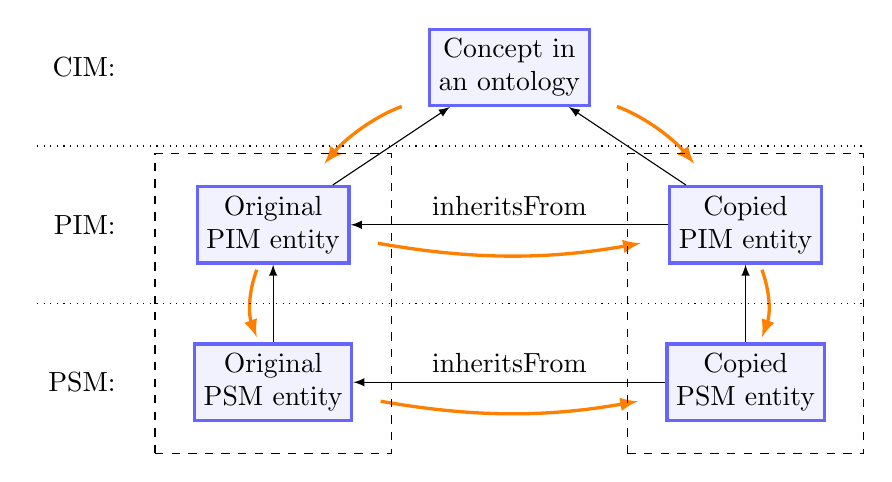
\begin{tikzpicture}[
        squarednode/.style={rectangle, draw=blue!60, fill=blue!5, very thick, minimum size=5mm,align=center},
    ]
        %Nodes
        \node[squarednode] (cim) at (0,0) {Concept in\\an ontology};
        \node[squarednode] (pim1) at (-3,-2) {Original\\PIM entity};
        \node[squarednode] (pimn) at (3,-2) {Copied\\PIM entity};

        \node[squarednode] (psma) at (-3,-4) {Original\\PSM entity};
        \node[squarednode] (psmb) at (3,-4) {Copied\\PSM entity};

        \node (psm_t)[text width=1cm,align=right] at (-5.5,0) {{CIM:}};
        \node (pim_t)[text width=1cm,align=right] at (-5.5,-2) {{PIM:}};
        \node (schema_t)[text width=1cm,align=right] at (-5.5,-4) {{PSM:}};

        %Lines
        \draw[-latex] (psma) -- (pim1);
        \draw[-latex] (psmb) -- (pimn);
        \draw[-latex] (pim1) -- (cim);
        \draw[-latex] (pimn) -- (cim);

        \draw[-latex] (pimn) -- node[above]{inheritsFrom} (pim1);
        \draw[-latex] (psmb) -- node[above]{inheritsFrom} (psma);


        \path(cim) edge [-latex,out=180+20, in=90-40,orange,shorten >=1em, shorten <=1em, very thick]  (pim1);
        \path(cim) edge [-latex,out=-20, in=90+40,orange,shorten >=1em, shorten <=1em, very thick]  (pimn);

        \path(pim1) edge [-latex,out=-10, in=180+10,orange,shorten >=1em, shorten <=1em, very thick]  (pimn);
        \path(psma) edge [-latex,out=-10, in=180+10,orange,shorten >=1em, shorten <=1em, very thick]  (psmb);

        \path(pim1) edge [-latex,out=270-20, in=90+20,orange,shorten >=.2em, shorten <=.2em, very thick]  (psma);
        \path(pimn) edge [-latex,out=270+20, in=90-20,orange,shorten >=.2em, shorten <=.2em, very thick]  (psmb);

        \node[dashed, draw=black, minimum width=3cm, minimum height=3.8cm] at (-3,-3) {};
        \node[dashed, draw=black, minimum width=3cm, minimum height=3.8cm] at (3,-3) {};

        % separators
        \foreach \x in {0,...,1}{
            \draw [dotted] (-6,-1-2*\x) -- (4.5,-1-2*\x);
        }
    \end{tikzpicture}
    \caption{Proposition on how to handle schema inheritance. PSM with PIM is copied and the links are preserved through inheritsFrom annotation. Possible evolution paths are denoted by orange arrows.} % Schema C shows a proposition for schema extending and is described later in the thesis.
\end{figure}
